\documentclass{beamer}

\usepackage[utf8]{inputenc}
\usepackage{hyperref}

\usetheme{Berkeley}
\beamertemplatenavigationsymbolsempty
\setbeamertemplate{headline}{}
 
\title{Importing data into FoodChain-Lab with All-in-one template}
\date{}
 
\begin{document}
\maketitle

\section{Tasks}
\begin{frame}
	\begin{itemize}
		\item In this tutorial we'll show you how to import delivery data to FoodChain-Lab via our All-in-one Excel template.
		\item All data will be entered in one file.
		\item The All-in-one template can be download from here: \url{https://github.com/SiLeBAT/BfROpenLabResources/raw/master/GitHubPages/templates/All_In_One_Template.xlsx}
	\end{itemize}
\end{frame}
 
\section{1}
\begin{frame}
	\begin{center}
  		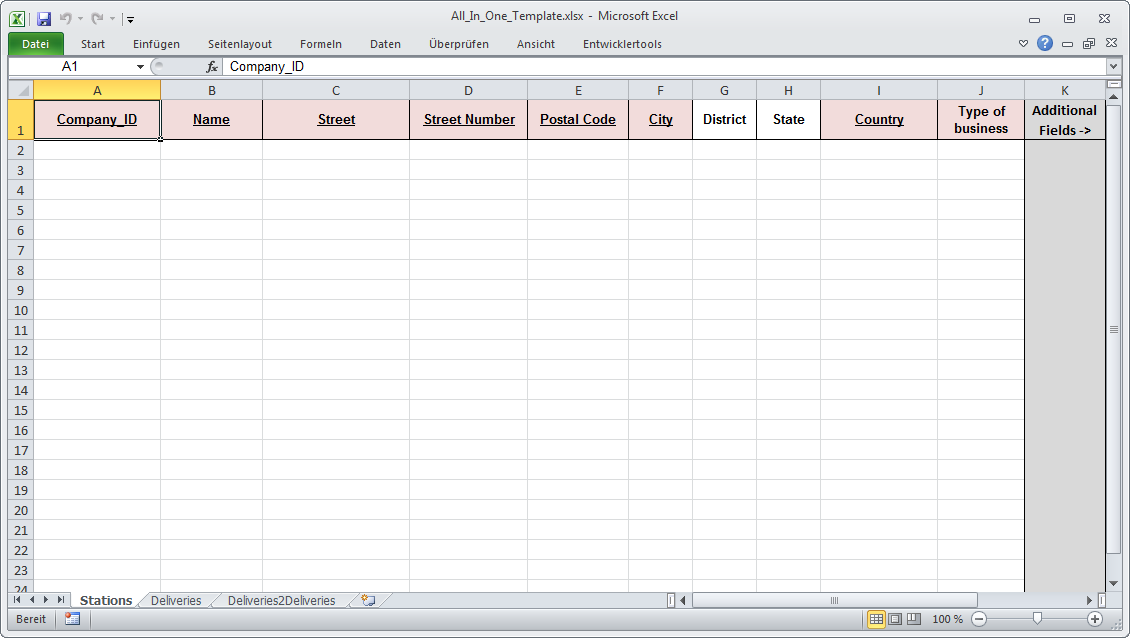
\includegraphics[height=0.5\textheight]{1.png}
	\end{center}
	\begin{itemize}
		\item Open "All\_In\_One\_Template.xlsx" and select the \textbf{Stations} sheet.
		\item Here you must enter all stations of the delivery network.
		\item The \textbf{Company\_ID} column is mandatory, all other columns are optional.
		\item Next to \textbf{Additional Fields} you can specify your own columns, for which you would like to enter data.
	\end{itemize}
\end{frame}

\section{2}
\begin{frame}
	\begin{center}
  		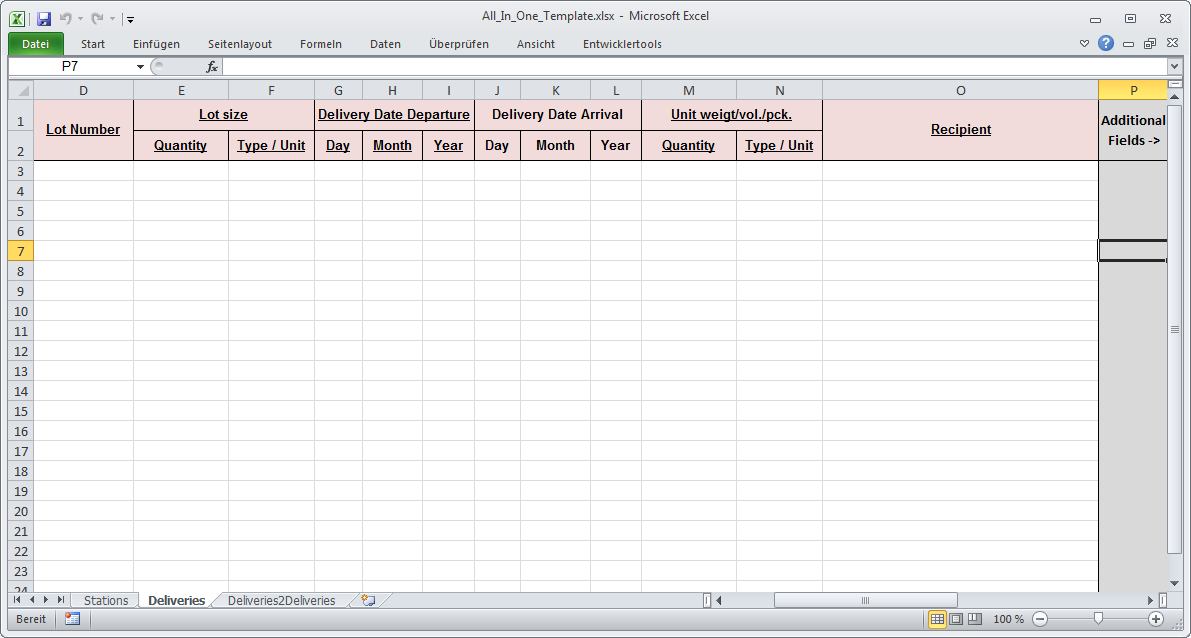
\includegraphics[height=0.5\textheight]{2.png}
	\end{center}
	\begin{itemize}
		\item Now select the \textbf{Deliveries} sheet.
		\item Here you must enter all deliveries between the stations defined in the previous sheet.
		\item The columns with the red headers are mandatory. In \textbf{Station} and \textbf{Recipient} you must enter \textbf{Company\_IDs} from the previous sheet.
		\item Next to \textbf{Additional Fields} you can specify your own columns, for which you would like to enter data.
	\end{itemize}
\end{frame}

\section{3}
\begin{frame}
	\begin{center}
  		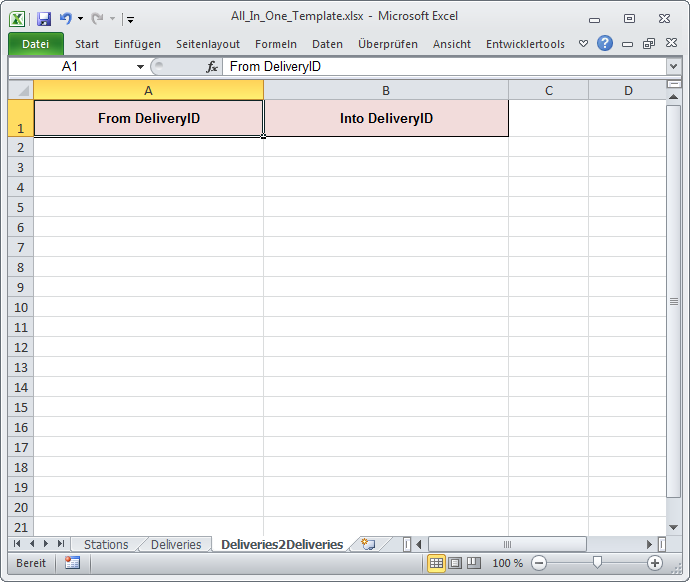
\includegraphics[height=0.6\textheight]{3.png}
	\end{center}
	\begin{itemize}
		\item Now select the \textbf{Deliveries2Deliveries} sheet.
		\item Here you can connect two deliveries from the previous sheet. In both columns you must enter \textbf{DeliveryIDs}.
		\item The \textbf{From}-delivery is a part/ingredient of the \textbf{To}-delivery. A contamination can spread from "\textbf{From}" to "\textbf{To}".
	\end{itemize}
\end{frame}

\section{4}
\begin{frame}
	\begin{center}
  		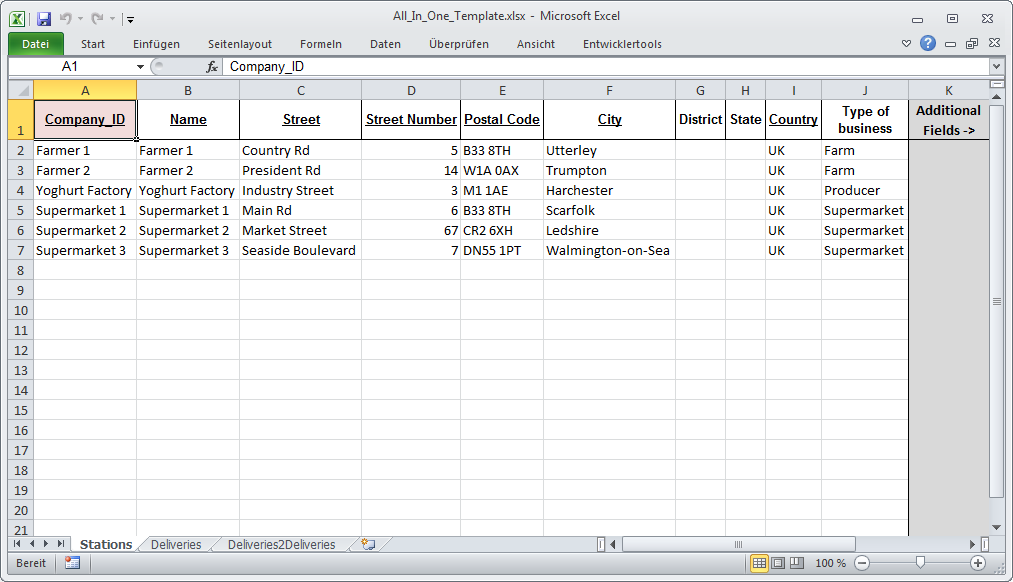
\includegraphics[height=0.6\textheight]{4.png}
	\end{center}
	\begin{itemize}
		\item Switch back to the \textbf{Stations} sheet and enter the data from the screenshot.
	\end{itemize}
\end{frame}

\section{5}
\begin{frame}
	\begin{center}
  		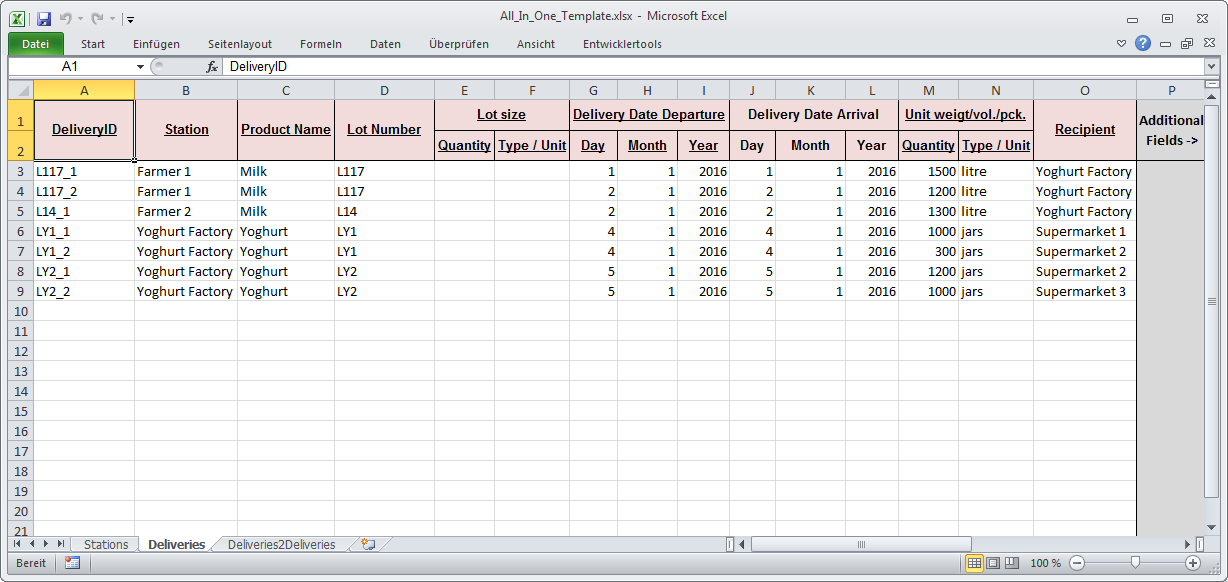
\includegraphics[height=0.5\textheight]{5.png}
	\end{center}
	\begin{itemize}
		\item Switch to the \textbf{Deliveries} sheet and enter the data from the screenshot.
		\item The "Yogurt Factory" produces two lots of yogurt. Milk from delivery "L117\_1" is used for the first lot ("LY1") and milk from deliveries "L117\_2" and "L14\_1" is used for the second lot ("LY2"). This ingredient information will be entered in the next sheet.
	\end{itemize}
\end{frame}

\section{6}
\begin{frame}
	\begin{center}
  		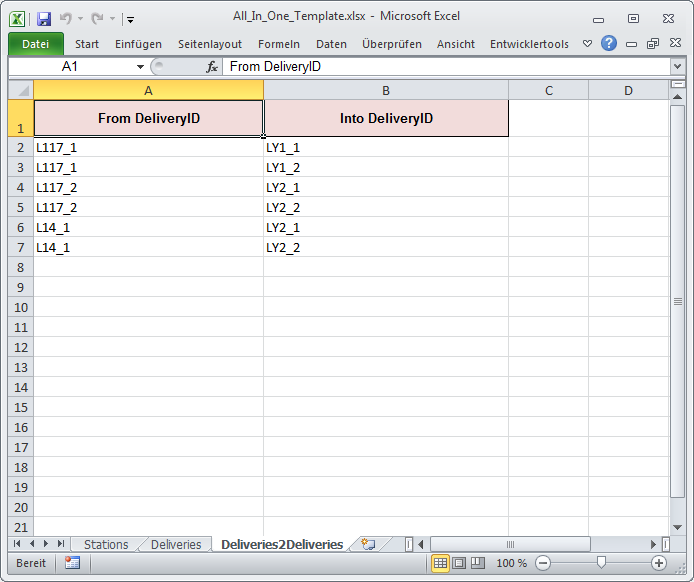
\includegraphics[height=0.6\textheight]{6.png}
	\end{center}
	\begin{itemize}
		\item In this sheet you can only reference deliveries and not lots.
		\item Therefore we have to connect "L117\_1" to both deliveries of lot "LY1" ("LY1\_1" and "LY1\_2").
		\item And "L117\_2" and "L14\_1" have to be connected to both deliveries of lot "LY2" ("LY2\_1" and "LY2\_2").
	\end{itemize}
\end{frame}

\section{7}
\begin{frame}
	\begin{center}
  		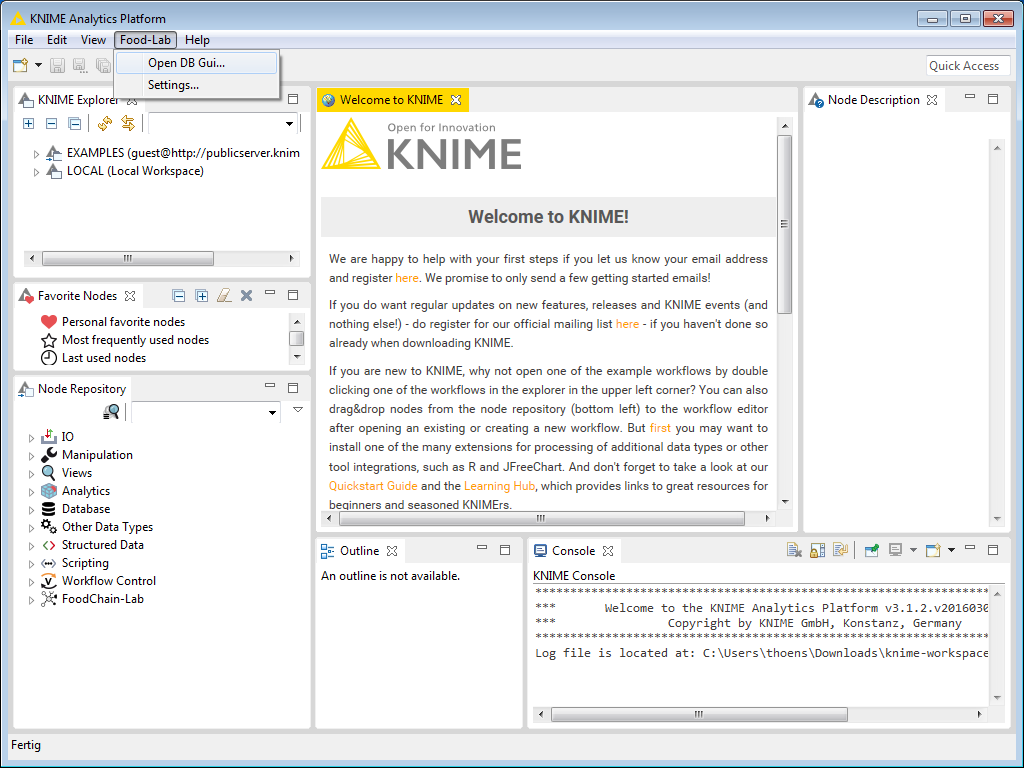
\includegraphics[height=0.6\textheight]{7.png}
	\end{center}
	\begin{itemize}
		\item After entering all data in the template, please open KNIME now.
		\item Then select \textbf{Food-Lab $>$ Open DB Gui...} in the menu bar to open the database interface.
	\end{itemize}
\end{frame}

\section{8}
\begin{frame}
	\begin{center}
  		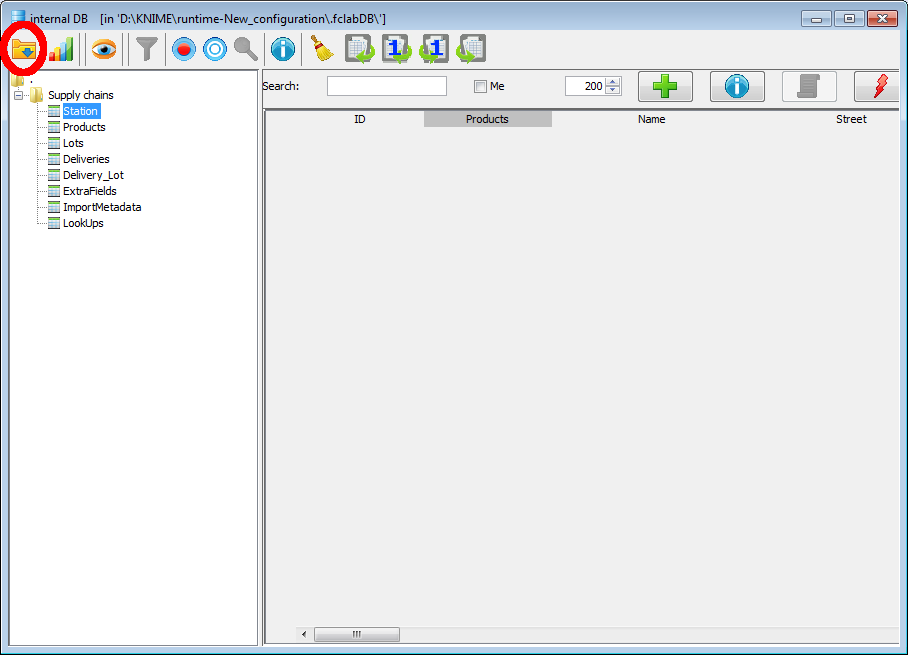
\includegraphics[height=0.6\textheight]{8.png}
	\end{center}
	\begin{itemize}
		\item To import this file click on the \textbf{Table import} button in the upper left corner of the database interface.
	\end{itemize}
\end{frame}

\section{9}
\begin{frame}
	\begin{center}
  		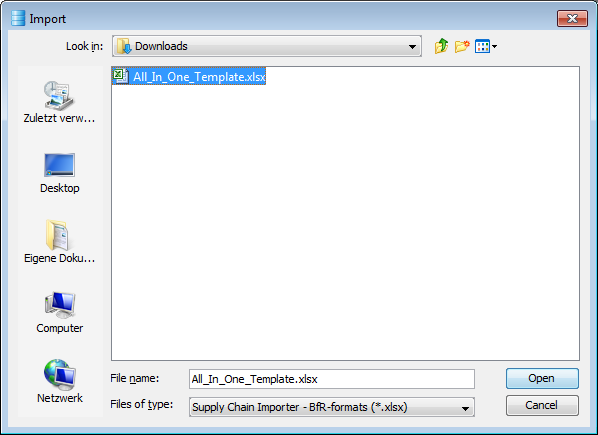
\includegraphics[height=0.5\textheight]{9.png}
	\end{center}
	\begin{itemize}
		\item In the file dialog that appears, select "All\_In\_One\_Template.xlsx" and press \textbf{Open}.
	\end{itemize}
\end{frame}

\section{10}
\begin{frame}
	\begin{center}
  		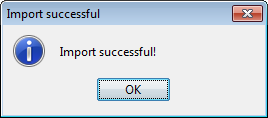
\includegraphics[width=0.4\textwidth]{10.png}
	\end{center}
	\begin{itemize}
		\item You'll see a message that the import was successful.
		\item Press \textbf{OK}.
	\end{itemize}
\end{frame}

\section{11}
\begin{frame}
	\begin{center}
  		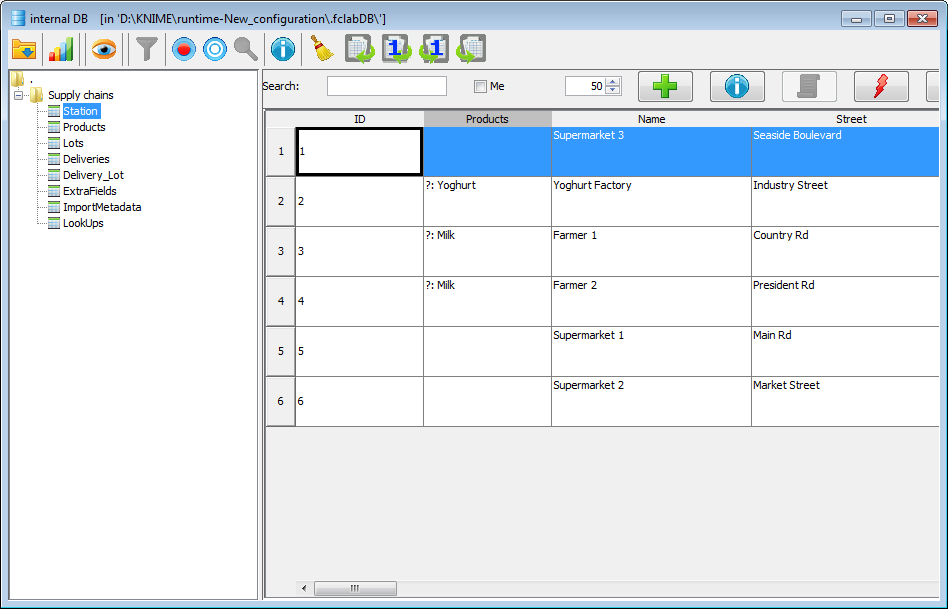
\includegraphics[height=0.5\textheight]{11.png}
	\end{center}
	\begin{itemize}
		\item In the database interface you'll notice, that there is now data in the tables.
	\end{itemize}
\end{frame}

\end{document}